%start preamble
\documentclass[paper=a4,fontsize=11pt]{scrartcl}%kind of doc, font size, paper size

\usepackage{fontspec}
\defaultfontfeatures{Ligatures=TeX}
%\setsansfont{Liberation Sans}
\usepackage{polyglossia}	
\setdefaultlanguage[spelling=new, babelshorthands=true]{german}
			
\usepackage{amsmath}%get math done
\usepackage{amsthm}%get theorems and proofs done
\usepackage{graphicx}%get pictures & graphics done
\graphicspath{{pictures/}}%folder to stash all kind of pictures etc
\usepackage{amssymb}%symbolics for math
\usepackage{amsfonts}%extra fonts
\usepackage{caption}%captions under everything
\usepackage{listings}
\numberwithin{equation}{section} 
\usepackage{float}%for garphics and how to let them floating around in the doc
\usepackage{xcolor}%nicer colors, here used for links
\usepackage{dsfont}
\usepackage{stmaryrd}
\usepackage{geometry}
\usepackage{hyperref}
\usepackage{fancyhdr}
\usepackage{multicol}
\usepackage{csquotes}
\usepackage{enumitem}
\usepackage{pythonhighlight}

\usepackage[backend=biber,style=alphabetic,
citestyle=alphabetic]{biblatex} %biblatex mit biber laden
\addbibresource{sources.bib}

%settings colors for links
\hypersetup{
    colorlinks,
    linkcolor={blue!50!black},
    citecolor={blue},
    urlcolor={blue!80!black}
}

\definecolor{pblue}{rgb}{0.13,0.13,1}
\definecolor{pgreen}{rgb}{0,0.5,0}
\definecolor{pred}{rgb}{0.9,0,0}
\definecolor{pgrey}{rgb}{0.46,0.45,0.48}


\pagestyle{fancy}
\lhead{NW+VS -- Übung\\WiSe 2021/22}
\rhead{FB 4 -- IKG \\ HTW-Berlin}
\lfoot{Übungsblatt 02 -- Application Layer}
\cfoot{}
\fancyfoot[R]{\thepage}
\renewcommand{\headrulewidth}{0.4pt}
\renewcommand{\footrulewidth}{0.4pt}

\lstdefinestyle{Bash}{
  language=bash,
  showstringspaces=false,
  basicstyle=\small\sffamily,
  numbers=left,
  numberstyle=\tiny,
  numbersep=5pt,
  frame=trlb,
  columns=fullflexible,
  backgroundcolor=\color{gray!20},
  linewidth=0.9\linewidth,
  %xleftmargin=0.5\linewidth
}

% Python style for highlighting
\newcommand\pythonstyle{\lstset{
language=Python,
basicstyle=\ttm,
morekeywords={self},              % Add keywords here
keywordstyle=\ttb\color{deepblue},
emph={MyClass,__init__},          % Custom highlighting
emphstyle=\ttb\color{deepred},    % Custom highlighting style
stringstyle=\color{deepgreen},
frame=tb,                         % Any extra options here
showstringspaces=false
}}


%%here begins the actual document%%
\newcommand{\horrule}[1]{\rule{\linewidth}{#1}} % Create horizontal rule command with 1 argument of height

\begin{document}
\begin{center}
\Large{\textbf{Übungsblatt 02 --  Application Layer}}
\end{center}

\begin{center}\Large{\textbf{Aufgabe A -- HTTP(S) \& HTML}}\end{center}\vskip0.25in
\begin{enumerate}
	\item Navigieren sie mithilfe der Kommandozeile in den \path{shell_tutorial} Ordner. Kopieren sie sie die Datei in \path{shell_tutorial.md} und bennen sie die Kopie in \emph{index.html} um.
	\item Wir gestalten im Folgenden eine kleine Website mit den Inhalten ihres Cheat-Sheets:
	\begin{enumerate}
		\item Öffnen sie die \path{index.html} mithilfe von \emph{vim}.
		\item Da die Website in \emph{HTML} gehalten ist, sollten wir dies festhalten. Mit dem Tag \texttt{<!DOCTYPE html>} in der ersten Zeile kann dies erfolgen. 
		\item Jedes weitere Tag muss einen Beginn und Ende haben. D.h. \texttt{<TAG>} setzt den Start und \texttt{</TAG>} setzt das Ende. Legen sie ein \texttt{html}-Tag an. Also \texttt{<html>} in die zweite Zeile und \texttt{</html>} in die letzte Zeile.
		\item Im Header werden Metainformationen festgehalten. Setzen sie ein Head-Tag. In das Head-Tag setzen sie ein Title-Tag.
		\item Der Body definiert den eigentliche Inhalt der Website, hier liegen die sichtbaren Inhalte. Legen sie einen Body um ihre genutzen Kommandos an.
		\item \texttt{<h1>} gibt Überschriften an, wobei \texttt{<h1>} die größtmögliche Überschrift ist.
		\item Mit \texttt{<p>} können Paragraphen angelegt werden.
		\item Mit \texttt{<br>} erzwingen sie eine Linebreak (Zeilenumbruch).
		\item Gestalten sie ihr Cheat-Sheet zu einer kleinen simplen Website.
		\item Überprüfen sie, ob ihr HTML alle notwendigen Tags des Listing aufweist:
		\begin{lstlisting}[style=Bash, language=Bash]
 <!DOCTYPE html>
<html>
<head>
<title>Page Title</title>
</head>
<body>

<h1>Shell Cheat Sheet</h1>
...
<h3>Basics</h1>
<p>ls</p>
ls -la <br>
ls -lisa <br>
...
<h3>vi/vim</h1>
</body>
</html> 
		\end{lstlisting}
	\end{enumerate}
	\item Python liefert ihnen eine rudimentären Webserver frei Haus. Starten sie im Ordner der \path{index.html} Datei folgendes Kommando:
		\begin{lstlisting}[style=Bash, language=Bash]
python3.8 -m http.server 8000
#Fuer die alte VM:
python3.7 -m http.server 8000
		\end{lstlisting}
	\item Rufen sie die Webseite mit \url{http://localhost:8000} im Browser auf.
	\item Folgendes kann beobachtet werden:
	\begin{figure}[H]
	\center
	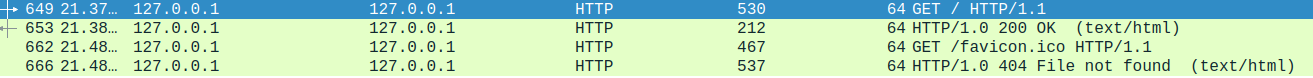
\includegraphics[scale=0.3]{get1}\\
	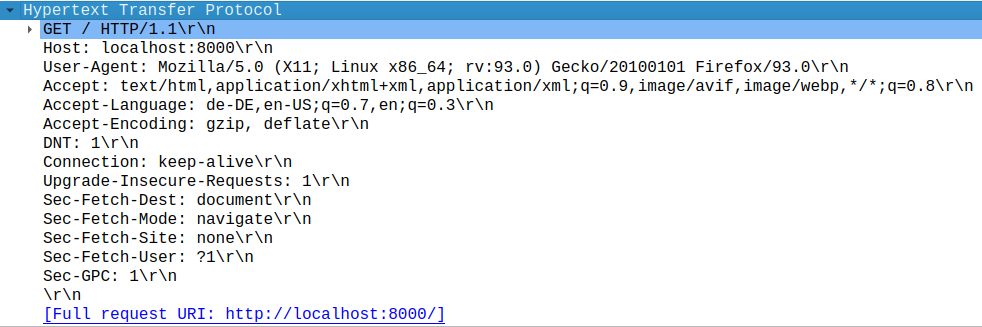
\includegraphics[scale=0.4]{get2}
	\end{figure}
	\begin{enumerate}
		\item Der Webserver arbeitet mit \emph{HTTP}. Zum abrufen einer HTTP-Anfrage wird die \emph{GET}-Methode genutzt. Lesen sie genau, wie der \emph{GET}-Request aussieht. Für uns sind die ersten zwei Zeilen.
		\item Auf den Request folgt die Antwort des Servers via \emph{HTTP}-Response.
		\begin{figure}[H]
		\center
		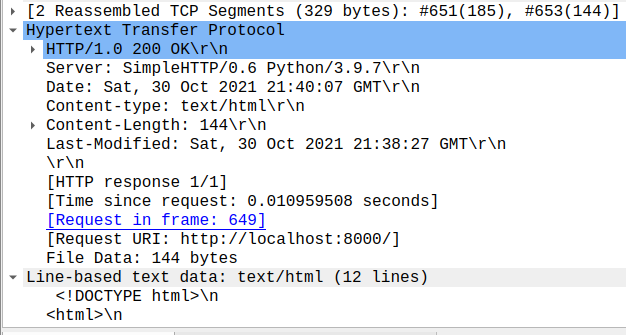
\includegraphics[scale=0.5]{get3}
		\end{figure}
		Lesen sie den Response genau.
	\end{enumerate}
	\item Verbinden sie sich nun via Kommandozeilen-Programm \emph{telnet} mit unserem lokalen \emph{HTTP}-Server.	
	\begin{lstlisting}[style=Bash, language=Bash]
telnet localhost 8000
\end{lstlisting}
	Mit \emph{telnet} können sie sich auf verschiedenste Server verbinden. Es dient hier lediglich, um eine Verbindung zum Webserver herzustellen.
	\item Nachdem die Verbindung hergestellt wurde wollen wir ein \emph{HTTP}-Request absetzen. Tippen sie die 
	ersten zwei Zeilen des \emph{GET}-Requests ab -- lassen sie jedoch die Zeichen \texttt{\textbackslash r\textbackslash n} weg.
	\item Wenn sie zu einem Server eine Verbindung aufbauen, wird serverseitig ein Timeout gestartet, so das, wenn nicht innerhalb einer gewissen Zeitspanne eine Anfrage kommt, der Server die Verbindung beendet. Wenn sie etwas umfangreichere Befehle an den Server senden müssen, oder das Ganze ohne manuellem Eintippen automatisieren wollen, können Sie das Tool \emph{netcat} nutzen.	
	\item Mit dem Werkzeug \emph{netcat} können Website direkt über die Kommandozeile aufgerufen werden.
	\begin{lstlisting}[style=Bash, language=Bash]
nc -v localhost 8000
\end{lstlisting}
	\begin{enumerate}
		\item Schreiben sie die gleichen HTTP-Befehle zum Abruf der Webseite jetzt in eine lokale Textdatei Diesmal.\\
		Dise können sie mithilfe der \emph{printf} Funktion beispielsweise lösen:
		\begin{lstlisting}[style=Bash, language=Bash]
printf "GET \ HTTP1.1 ..." > request
printf "GET / HTTP/1.1\nHOST: localhost:8000\n\n"
cat request | nc localhost 8000
\end{lstlisting}
		Alternativ könne sie dies auch via \emph{vim} erledigen.
		\item Lassen sie sich den Inhalt der Datei auf der Kommandozeile nach Std-Out ausgeben (\emph{cat}).
		\item Leiten sie diese Ausgabe mittels einer \emph{Pipe} (\path{|}) als Eingabe in den Befehl \emph{netcat} um. Rufen sie \emph{netcat} dabei mit Parametern so auf, dass es eine Verbindung wieder zum gleichen Webserver und Port wie bisher aufbaut.\\
		Wenn sie alles richtig gemacht haben, sehen sie wieder die gleiche Ausgabe.
	\end{enumerate}
\end{enumerate}

\newpage

\begin{center}\Large{\textbf{Aufgabe B -- Python}}\end{center}\vskip0.25in
\begin{enumerate}
	\item Starten sie eine interaktive Python-Session.
	\begin{lstlisting}[style=Bash, language=Bash]
python
\end{lstlisting}
	\item Python als Taschenrechner.
	\begin{enumerate}
	\item Berechnen sie folgende Terme:
		\begin{itemize}
			\item $2 + 3$
			\item $3.5 + 4.5$
			\item $3 + 3.5$
		\end{itemize}
		Lassen sie sich mit \emph{type()} den jeweiligen Datentyp ausgeben.
		\item Deklarieren sie folgende Variablen:
		\begin{itemize}
			\item Variable $a$ mit Wert $2$
			\item Variable $b$ mit Wert $3$
			\item Variable $c$ als Summe von $a$ und $b$
			\item Eine Variable $s1$ die den Inhalt: \emph{Netzwerke} und eine Variable $s2$ mit dem Inhalt \emph{verteilte Systeme} enthält.
			\item Fügen sie in der Variablen $s$ die beiden Texte $s1, s2$ mit dem $+$ Operator zusammen.
		\end{itemize}
	\end{enumerate}
	\item Mithilfe der \emph{print()} Funktion können Ausgaben auf der Kommandozeile ausgegeben werden.
	\begin{enumerate}
		\item \enquote{printen} sie die Zeile \enquote{Hallo, Welt!} auf der Kommandozeile.
	\end{enumerate}
	\item Kontrollstrukturen:
	\begin{python}
if x % 2:
	print("x is even")
else:
	print("x is odd")
\end{python}
	\begin{enumerate}
		\item Schreiben und testen sie eine Block der prüft, ob zwei Variablen numerisch identisch sind (\enquote{$==$}). 
		\item Schreiben und testen sie eine Block der eine Ausgabe ausführt, wenn die erste Variable größer als die zweite ist.
	\end{enumerate}
	\item For-Schleifen:
\begin{python}
for i in range(X) # X ist hier die Anzahl der Wiederholungen
\end{python}
	\begin{enumerate}
		\item Schreiben und testen sie mithilfe eine For-Schleife, die ihnen 10 mal \enquote{Hallo, Welt!} ausgibt.
		\item Schreiben und testen sie mithilfe einer For-Schleife die Gaußsche Summenformel. Also die Summe der Zahlen von $0$ bis $m$
		$$ 0 + 1 + 2 + ... + m = \sum_{k=0}^m k$$
	\end{enumerate}
\item While-Schleifen:
\begin{python}
while i <= n: # X ist hier die Anzahl der Wiederholungen
\end{python}
	\begin{enumerate}
	\item Schreiben sie eine \emph{While}-Schleife, die alle Zahlen kleiner der Variablen $c$ nacheinander ausgibt.
	\end{enumerate}
	\item Funktionen
	\begin{python}
	def foo(): # Funktion ohne Argument
	def bar("Blub"): #Funktion mit Argument hard coded
	def bar2(m): Funktion mit Argument als Variable
	def square(x): # Funktion mit Argument und Rückgabewert
		return x**2
	\end{python}
\begin{enumerate}
	\item Schreiben sie eine Funktion \texttt{euclid} die den euklidischen Algorithmus implementiert. Nutzen sie eine Funktiosdeklaration.
\end{enumerate}
\end{enumerate}

\end{document}
